\documentclass[10pt,a4paper]{article}
\usepackage[utf8]{inputenc}
\usepackage[T1]{fontenc}
\usepackage{amsmath}
\usepackage{amsfonts}
\usepackage{amssymb}
\usepackage{graphicx}
\usepackage{indentfirst}
\usepackage{etoolbox}
\usepackage{placeins}
\usepackage{subcaption}
\usepackage{gensymb}

\usepackage[style=ieee, backend=bibtex ,sorting=none]{biblatex}
\addbibresource{refs.bib}
%opening
\author{Piotr Kumala}
\title{Zastosowanie rekurencyjnych sieci neuronowych do predykcji szeregów czasowych}
\date{}
\graphicspath{ {./img/} }
\renewcommand*\contentsname{Spis treści}
\renewcommand*\figurename{Rysunek}

\begin{document}
\begin{titlepage}
	\begin{center}
		
\includegraphics[width=0.4\textwidth]{img/university.jpg}
		\vspace*{1cm}
		
		{\Huge
			\textbf{Praca magisterska} \\
			
		}
		\vspace{0.5cm}
		{\Large
			Zastosowanie rekurencyjnych sieci neuronowych do predykcji szeregów czasowych
			
			\vspace{1cm}
			
			\textbf{Piotr Kumala} \\
		}
		\vspace{0.5cm}
		kierunek studiów: \textbf{Informatyka Stosowana} \\
		
		\vspace{1cm}
		
		{\Large Opiekun: \textbf{dr hab. inż. Piotr A. Kowalski}}
		\vfill
		
		\
		\vspace{0.8cm}
		
		
		Wydział Fizyki i Informatyki Stosowanej\\
		Akademia Górniczo-Hutnicza im. Stanisława Staszica\\
		Kraków, lipiec 2021r.
		
	\end{center}
\end{titlepage}
\pagenumbering{gobble}
\newpage
\begin{center}
	\textbf{Oświadczenie studenta}
\end{center}

Uprzedzony o odpowiedzialności karnej na podstawie art. 115 ust. 1 i 2 ustawy z dnia
4 lutego 1994 r. o prawie autorskim i prawach pokrewnych (t.j. Dz. U. z 2018 r. poz. 1191 z
późn. zm.): „Kto przywłaszcza sobie autorstwo albo wprowadza w błąd, co do autorstwa całości
lub części cudzego utworu albo artystycznego wykonania, podlega grzywnie, karze
ograniczenia wolności albo pozbawienia wolności do lat 3. Tej samej karze podlega, kto
rozpowszechnia bez podania nazwiska lub pseudonimu twórcy cudzy utwór w wersji
oryginalnej albo w postaci opracowania, artystyczne wykonanie albo publicznie zniekształca
taki utwór, artystyczne wykonanie, fonogram, wideogram lub nadanie.”, a także uprzedzony o
odpowiedzialności dyscyplinarnej na podstawie art. 307 ust. 1 ustawy z dnia 20 lipca 2018r.
Prawo o szkolnictwie wyższym i nauce (Dz. U. z 2018 r. poz. 1668 z późn. zm.) „Student
podlega odpowiedzialności dyscyplinarnej za naruszenie przepisów obowiązujących w uczelni
oraz za czyn uchybiający godności studenta.”, oświadczam, że niniejszą pracę dyplomową
wykonałem osobiście i samodzielnie i nie korzystałem ze źródeł innych niż wymienione w
pracy. 

Jednocześnie Uczelnia informuję, że zgodnie z art. 15a ww. ustawy o prawie autorskim
i prawach pokrewnych Uczelni przysługuje pierwszeństwo w opublikowaniu pracy
dyplomowej studenta. Jeżeli Uczelnia nie opublikowała pracy dyplomowej w terminie 6
miesięcy od dnia jej obrony, autor może ją opublikować chyba, że praca jest częścią utworu
zbiorowego. Ponadto Uczelnia, jako podmiot, o którym mowa w art. 7 ust. 1 pkt 1 ustawy z
dnia 20 lipca 2018 r. — Prawo o szkolnictwie wyższym i nauce (Dz. U. z 2018 r. poz. 1668 z
późn. zm.), może korzystać bez wynagrodzenia i bez konieczności uzyskania zgody autora z
utworu stworzonego przez studenta w wyniku wykonywania obowiązków związanych z
odbywaniem studiów, udostępnić utwór ministrowi właściwemu do spraw szkolnictwa
wyższego i nauki oraz korzystać z utworów znajdujących się w prowadzonych przez niego
bazach danych, w celu sprawdzania z wykorzystaniem systemu antyplagiatowego. Minister
właściwy do spraw szkolnictwa wyższego i nauki może korzystać z prac dyplomowych
znajdujących się w prowadzonych przez niego bazach danych w zakresie niezbędnym do
zapewnienia prawidłowego utrzymania i rozwoju tych baz oraz współpracujących z nimi
systemów informatycznych.

\vfill
\
\begin{flushright}
	............................................................... \\
	(czytelny podpis)
\end{flushright}

\newpage
\pagenumbering{arabic}
\tableofcontents
\newpage

\section{Wprowadzenie i cel pracy}

\subsection{Wprowadzenie}
Sieci neuronowe są coraz powszechniej używane do rozwiązywania wielu problemów życia codziennego. Nawet w wydawałoby się prostych urządzeniach jak telefony komórkowe zawierane są układy elektroniczne specjalizujące się w obliczeniach korzystających z sieci neuronowych \cite{appleNeuralEngine}. Taki rozwój technologiczny może zostać zastosowany do próby zrozumienia i szukania rozwiązań problemów życia codziennego. Jednym z szeroko występujących w świadomości społecznej problemów jest poziom zanieczyszczenia środowiska naturalnego i zmiany klimatu. Co roku na początku zimy media raportują o wysokim poziome zanieczyszczeń powietrza w polskich miastach. Podejmowane są również działania mające na celu ograniczenie poziomu tychże zanieczyszczeń przez samorządy i instytucje centralne. Posiadanie wiarygodnych estymacji skali problemu i jego zmiany w czasie może mieć wymierne skutki w usprawnianiu reakcji na wysokie poziomy zanieczyszczeń. W tej pracy podjęta zostanie próba stworzenia wiarygodnego modelu predykcyjnego poziomu zanieczyszczeń korzystającego z rekurencyjnych sieci neuronowych.

\subsection{Cel pracy}
Rekurencyjne sieci neuronowe są szeroko wykorzystywane i rozwijane przez największe firmy technologiczne. Są one stosowane między innymi do rozpoznawania pisma odręcznego i tekstu dyktowanego (Google Android LSTM). Mając na uwadze ilość wysiłku wkładanego w ulepszanie tychże sieci nasuwa się pytanie jakie rezultaty będą one osiągać w innych zastosowaniach. W ramach tej pracy zbadana zostanie jakość predykcji szeregów czasowych płynących z modeli opartych na rekurencyjnych sieciach neuronowych. Zostaną one zestawione z klasycznymi metodami predykcyjnymi w celu stwierdzenia zasadności stosowania sieci neuronowych. Specjalna uwaga zostanie również poświęcona różnicom w jakości uzyskiwanych rozwiązań różnych architektur sieci oraz skalowalności modeli opartych na rekurencyjnych sieciach neuronowych. 

\section{Wstęp teoretyczny}
\subsection{Szereg czasowy}
W ramach pracy podejmowane będą próby predykcji szeregu czasowego. Przed rozpoczęciem dalszych dywagacji należy zdefiniować samo pojęcie aby uniknąć nieścisłości. Podążając za Głównym Urzędem Statystycznym szeregiem czasowym nazywamy ciąg obserwacji ilustrujący kształt zjawiska w kolejnych okresach czasu. Obserwacją można określić zbiór cech opisujących zjawisko w danym punkcie czasu. Rozumiejąc w taki sposób pojęcie szeregu czasowego można w prosty sposób określić cel systemu predykcyjnego. System ten powinien być w stanie przewidzieć wartość pewnej cechy w kolejnym punkcie czasu na podstawie poprzednich obserwacji. Można również określić, że predykcja będzie tym lepsza im bardziej zgodna z posiadanymi obserwacjami. 

\subsection{Regresja liniowa}
Jedną z najbardziej klasycznych metod predykcyjnych jest regresja liniowa. Jej podstawy zostały położone w pracach Legrende'a i Gauss'a na początku XIX wieku \cite{seal1967studies}. Polega ona na dopasowywaniu funkcji liniowej do danych w taki sposób, aby jak najlepiej opisywała ona kształt i właściwości danych. Najprostszym mechanizmem służącym do zapewnienia optymalnych wyników jest metoda najmniejszych kwadratów opisana po raz pierwszy przez Legrende'a w 1805 roku\cite{legendre1806nouvelles}. Polega ona na takim dopasowywaniu parametrów funkcji aby zminimalizować sumaryczny kwadrat odległości obserwacji od prostej opisanej funkcją. 
\begin{figure}[!ht]
	\centering
	\makebox[0pt]{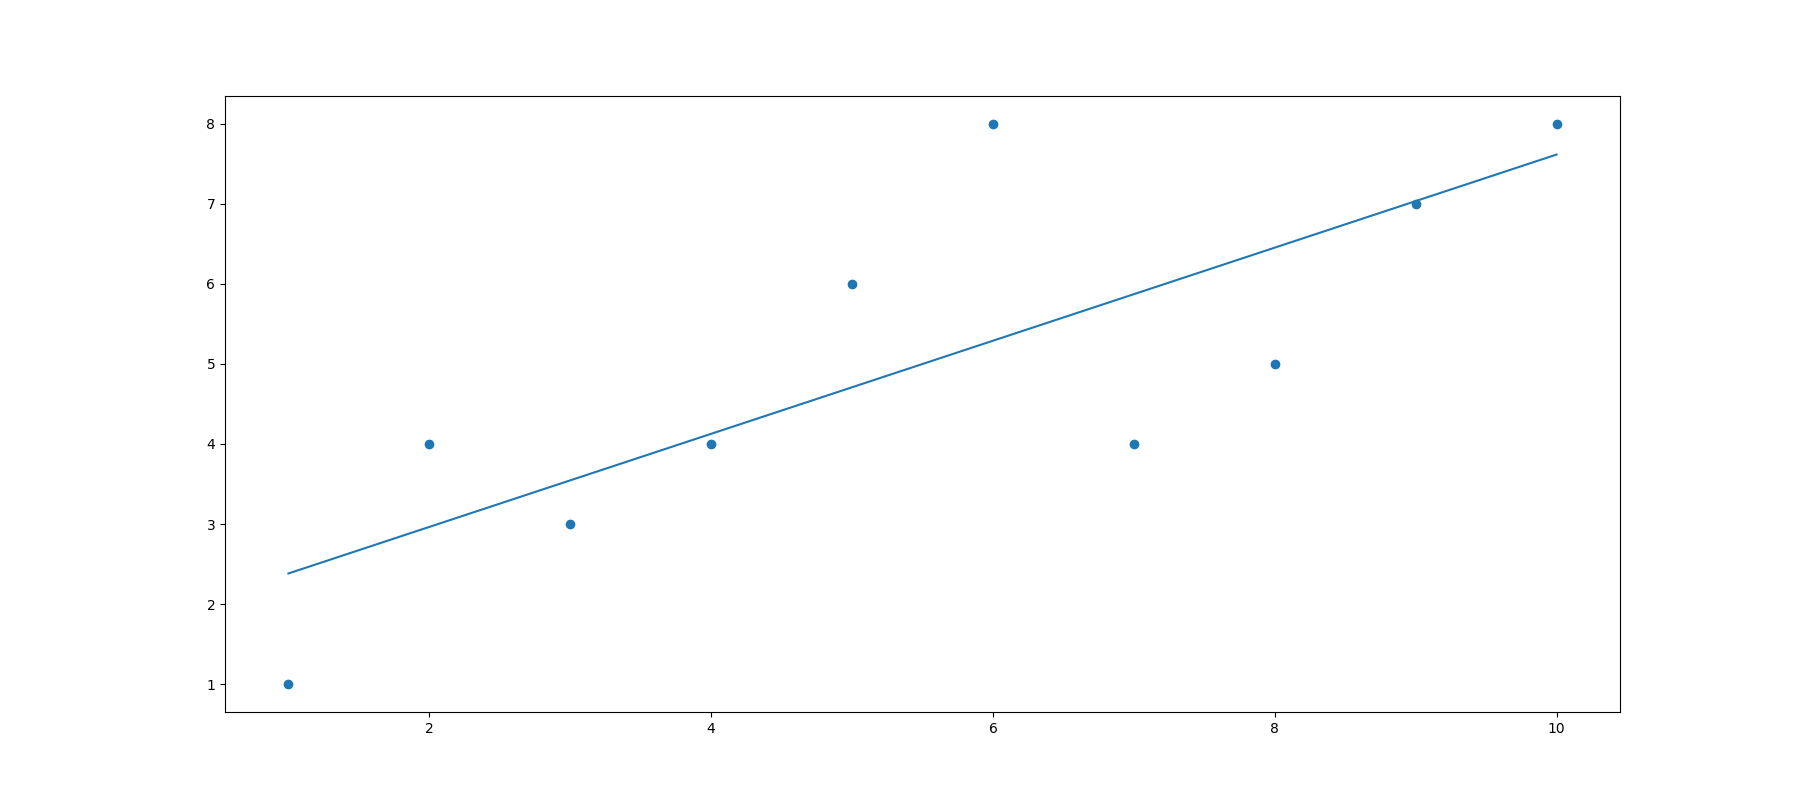
\includegraphics[scale=0.2]{example_linear_regression.png}}
	\caption{Przykład wyniku regresji liniowej}
\end{figure}
\FloatBarrier
Metoda ta jest szeroko wykorzystywana, ale nie jest pozbawiona wad. Bardzo mocno reaguje ona na elementy nietypowe co może prowadzić do nieprawidłowego kształtu funkcji. F. Anscombe  w 1973 roku zaprezentował cztery zbiory danych, które korzystając z metody najmniejszych kwadratów zwracają takie same proste pomimo tego, że kształty tychże zbiorów danych są bardzo od siebie różne \cite{anscombe1973graphs}.
\begin{figure}[!ht]
	\centering
	\makebox[0pt]{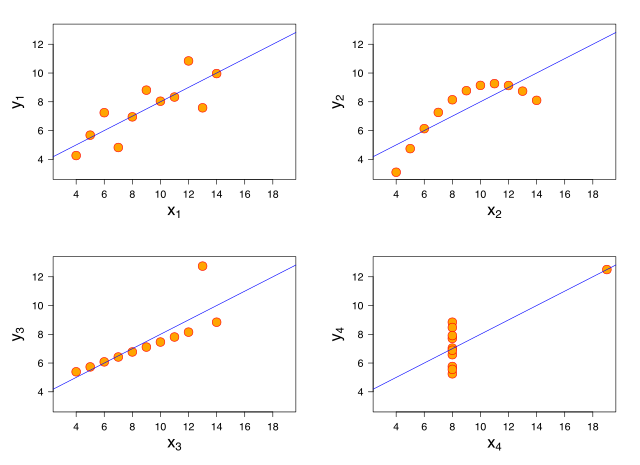
\includegraphics[scale=0.6]{anscombe.png}}
	\caption{Zbiory opisane przez Anscombe'ego i dopasowane do nich proste}
\end{figure}
\FloatBarrier 
\subsection{Drzewa decyzyjne}
Jedną z najszerzej używanych metod uczenia maszynowego są drzewa decyzyjne. Są one szeroko wykorzystywane ze względu na swoje nieskomplikowanie i intuicyjność w zrozumieniu wyników \cite{wu2008top}. Drzewem decyzyjnym nazywamy model predykcyjny, $h: X \rightarrow Y$, który przewiduje wartość $Y$ dla $x$ poprzez trawers drzewa od korzenia do liścia. Na każdym węźle drzewa kierunek przejścia jest wybierany poprzez rozdzielenie przestrzeni wejściowej. Najczęściej jest ono dokonywane na podstawie cech obserwacji $x$ \cite{books/daglib/0033642}. Wynikiem procesu uczenia jest drzewo pozwalające prześledzić ścieżkę jaką podąża każda obserwacja $x$ w celu przypisania jej odpowiedniej wartości. Przykładowe, bardzo uproszczone drzewo decyzyjne jest przedstawione na rysunku numer 3.
\begin{figure}[!ht]
	\centering
	\makebox[0pt]{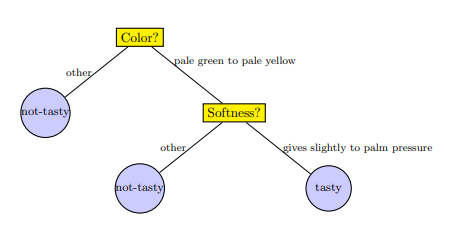
\includegraphics[scale=0.8]{example_decission_tree.png}}
	\caption{Przykładowe drzewo decyzyjne}
\end{figure}
\FloatBarrier

Na podstawie tego przykładu można łatwo zaobserwować główną zaletę drzew decyzyjnych, mianowicie łatwość interpretacji uzyskanego drzewa. Podejmowanie decyzji poprzez odpowiadanie na pytania, które stale zawężają możliwe rozwiązania jest intuicyjnie zrozumiałe. Powodem tej łatwości zrozumienia może być bliskość procesu wyboru przez drzewo do ludzkiego procesu podejmowania decyzji. Niektórzy ludzie twierdzą, że drzewo decyzyjne powiela ludzkie schematy myślowe \cite{James2013}. 

Drzewa decyzyjne mogą być wykorzystywane w problemach regresyjnych to znaczy dla ciągłej dziedziny rozwiązań $Y$. Należy jednak pamiętać, że w takim przypadku  należy uważać na możliwość zbytniego dopasowywania drzewa do danych trenujących. Problem ten objawia się stworzeniem zbyt szczegółowego drzewa, które nie generalizuje odpowiednio danych nieobecnych w zbiorze treningowym.

\subsection{Rekurencyjne sieci neuronowe}
Rekurencyjne sieci neuronowe to sieci neuronowe posiadające pętlę sprzężenia zwrotnego w swojej warstwie rekurencyjnej. Taka struktura pozwala im ,,zapamiętywać'' informacje przez pewien okres czasu i wykorzystywać w dalszych predykcjach \cite{reviewOfANN2018}. Taka umiejętność pozwala przewidywać, że rekurencyjna sieć neuronowa powinna dobrze zachowywać się w predykcji szeregu czasowego dzięki ,,zapamiętywaniu'' wartości w poprzednich krokach czasowych. 

Podwaliny rekurencyjnych sieci neuronowych zostały stworzone w 1986 roku przez D. Rumelhart'a. Opisywał on sposób uczenia sieci neuronowych poprzez propagację wsteczną błędu \cite{rumelhart1986learning}. Zauważył on, że korzystając z tej metody uczenia można wypracować sieć, która rekurencyjnie wyznaczy wartości wag neuronów w swojej warstwie ukrytej. Potrzeba opracowania nowego sposobu uczenia wynikała z istnienia zadań niedających się rozwiązać poprzez proste połączenie jednostek wejściowych z wyjściowymi.

Powszechnym sposobem myślenia o strukturze sieci neuronowych jest seria warstw składających się na sieć. Każda warstwa składająca się z pewnej liczby neuronów komunikuje się z następującą warstwą aż do osiągnięcia warstwy wyjściowej zwracającej wynik sieci. 
\begin{figure}[!ht]
	\centering
	\makebox[0pt]{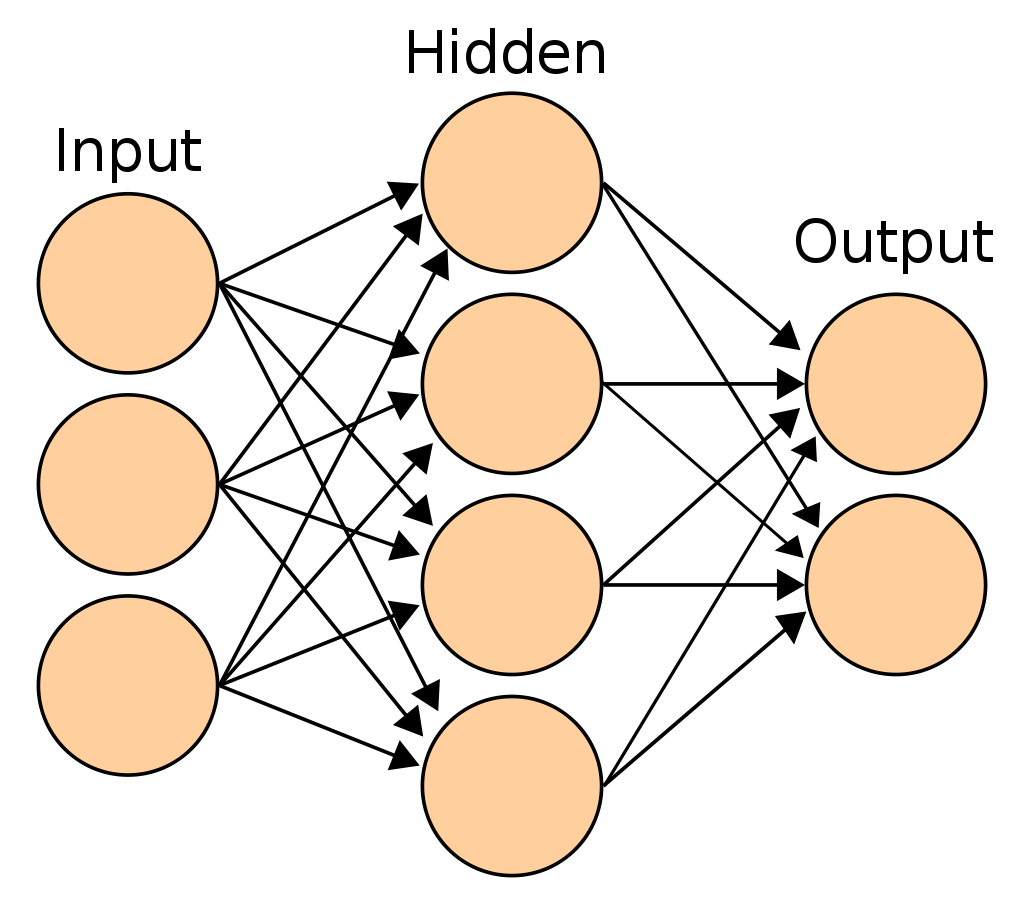
\includegraphics[scale=0.3]{ann_layers.png}}
	\caption{Przykładowa sieć neuronowa z trzema warstwami}
\end{figure}
\FloatBarrier

W przypadku sieci rekurencyjnej nie jest tworzona seria warstw komunikujących się ze sobą, a jedna rekurencyjna warstwa zmieniająca się w czasie. W celu lepszego zrozumienia struktury i sposobu działania takiej sieci często dokonywany jest proces rozwijania w czasie warstwy rekurencyjnej.

\begin{figure}[!ht]
	\centering
	\makebox[0pt]{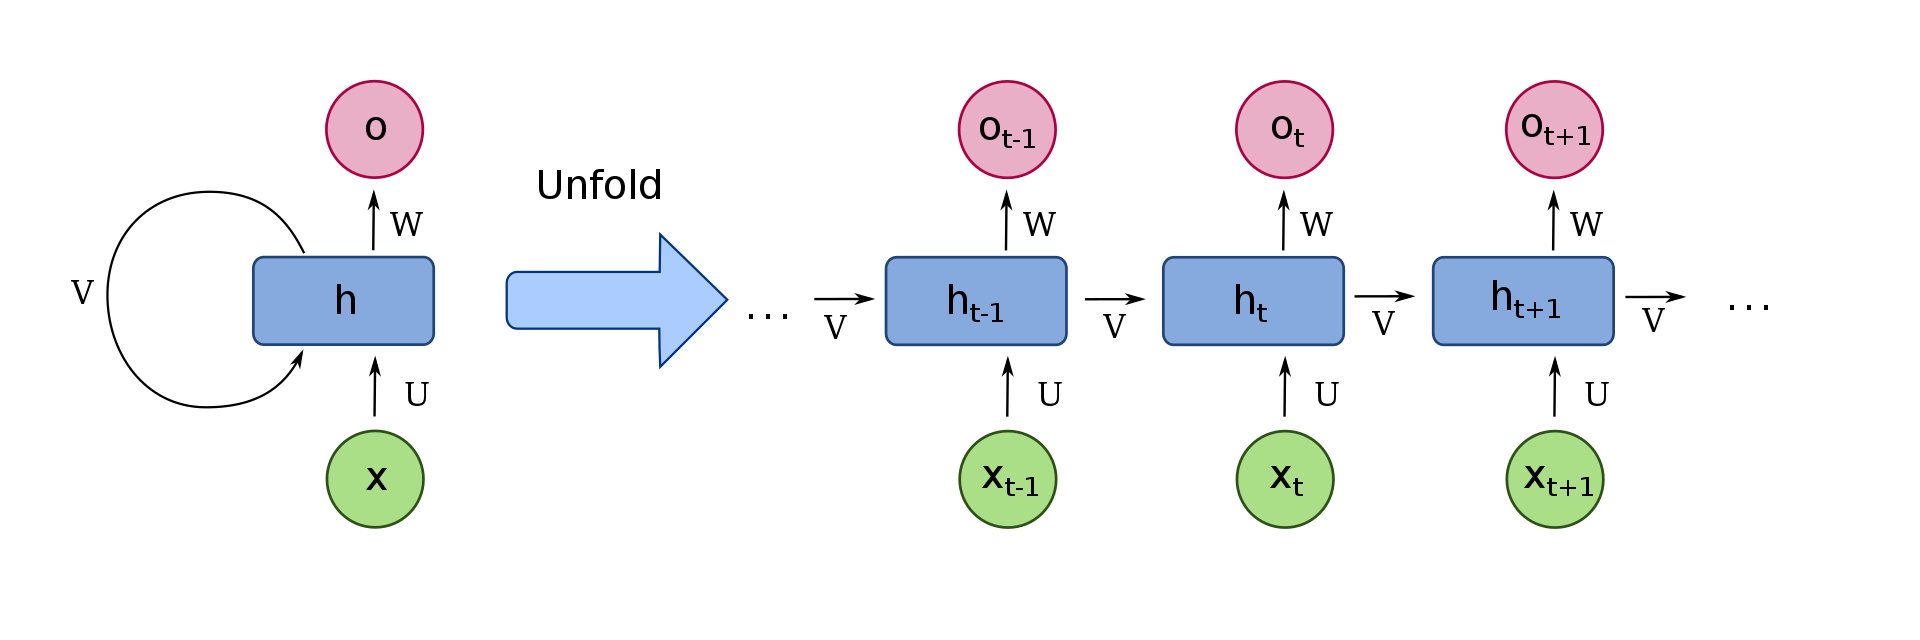
\includegraphics[scale=0.3]{Recurrent_neural_network_unfold.png}}
	\caption{Przykład rozwijania warstwy rekurencyjnej $h$}
\end{figure}
\FloatBarrier

W powyższym przykładzie należy zauważyć, że w wersji rozwiniętej $h_{t-1}, h_t i h_{t+1}$ nie są osobnymi warstwami, a jedynie reprezentacją warstwy $h$ w różnych krokach czasowych. 

Na przestrzeni lat powstało wiele wariacji na temat architektury rekurencyjnych sieci neuronowych odpowiadających na różne problemy i wymagania im stawiane. W dalszym ciągu pracy przedstawione zostaną wybrane architektury, które mogą zostać wykorzystane do rozwiązania postawionego problemu predykcji szeregu czasowego.


\subsection{Architektura LSTM}
Sieci Long Short-Term Memory(LSTM) powstały jako próba rozwiązania problemów występujących w klasycznych sieciach rekurencyjnych. Problemy te głównie dotyczyły aspektu rekurencyjnych sieci neuronowych pozwalającego ,,zapamiętać'' sieci poprzednie kroki czasowe. Zauważono, że korzystając z mechanizmu propagacji wstecznej przesyłany do następnych kroków czasowych sygnał błędu (sposób sieci na ,,zapamiętanie'' poprzednich przypadków) ma tendencję do znikania lub wybuchania. 

Zniknięciem sygnału błędu nazwać można sytuację, w której dąży on do zera w kolejnych krokach czasowych. Jest ona problemem w procesie uczenia, ponieważ może doprowadzić do bardzo dużego przedłużenia procesu lub nawet całkowicie uniemożliwić poprawne nauczenie sieci.

Wybuchem sygnału błędu nazywana jest sytuacja, w której dąży on do nieskończoności. Sytuacja ta jest niepożądana, ponieważ bardzo duży błąd przesyłany do następnych kroków czasowych oznacza, że sieć tak naprawdę niczego nie ,,zapamiętuje''. Może to prowadzić do oscylacji wag w sieci bez sygnału błędu stabilizującego wynik. 

Problemy te zostały podniesione przez S. Hochreiter'a w jego pracy doktorskiej, a następnie dokładniej opisane w roku 1991 we wspólnej pracy z J. Schmidhuber'em. 
W ramach artykułu ,,Long Short-Term Memory'' zaproponowali oni całkowicie nową architekturę rekurencyjnej sieci neuronowej dążącą do rozwiązania wyżej opisanych problemów \cite{hochreiter1997long}.

Stworzona została architektura oparta na komórkach pamięci i bramkach. Podstawową składową warstwy w tej architekturze jest komórka pamięci. Trzonem komórki jest rekurencyjna jednostka liniowa posiadająca Stałą Karuzelę Błędu (Constant Error Carousel), w skrócie CEC. Wartości CEC będą nazywane stanem komórki. Istnienie mechanizmu CEC eliminuje problemy z sygnałem błędu, ponieważ zapewnia on, że lokalny błąd nie będzie się samoistnie zmieniał w kolejnych krokach czasowych.

Mechanizmem odpowiedzialnym za modyfikację stanu komórki są bramki wejściowa i wyjściowa. Bramka wejściowa zajmuje się kontrolą przepływu nowych informacji do komórki. Oznacza to, że decyduje ona czy zachować obecny stan, czy nadpisać go nowymi informacjami. Można rozumieć zadanie bramki wejściowej jako określanie czy należy zapamiętać nową wiedzę lub uaktualnić istniejącą wiedzę. 

Bramka wyjściowa natomiast kontroluje przepływ stanu komórki na zewnątrz. Decyduje ona czy przechowywana przez komórkę wiedza jest warta przekazania innym komórkom do zapamiętania. Jej zadanie możemy rozumieć jako decyzję czy podzielić się swoją wiedzą z resztą komórek czy zachować ją dla siebie. 

\begin{figure}[!ht]
	\centering
	\makebox[0pt]{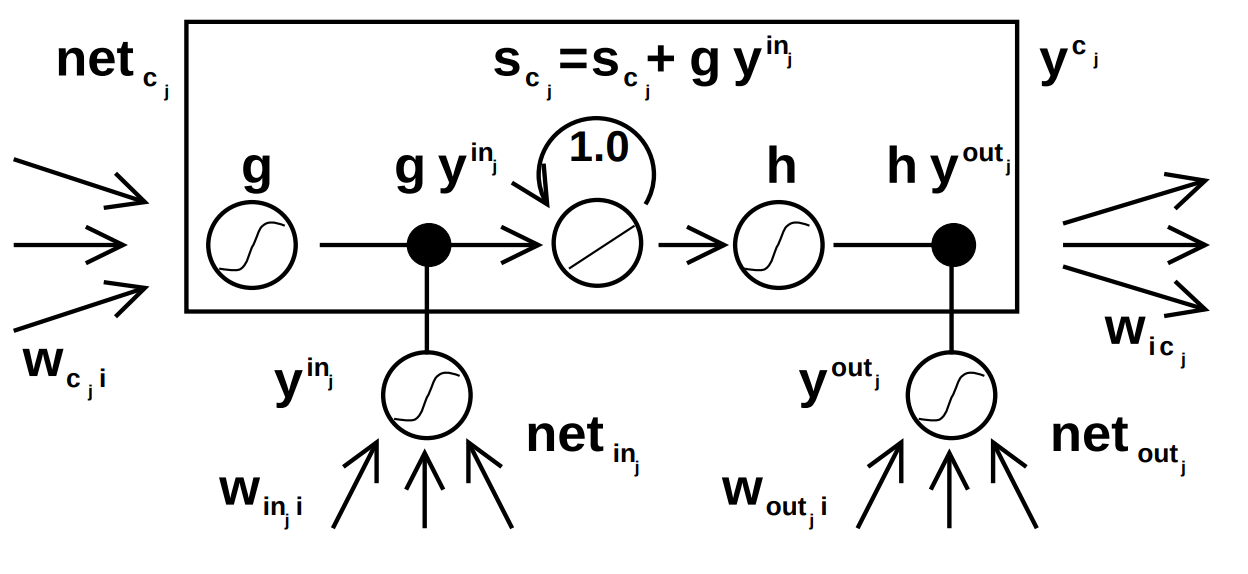
\includegraphics[scale=0.4]{lstm_without_forget_gate_schema.png}}
	\caption{Komórka pamięci w architekturze LSTM}
\end{figure}
\FloatBarrier

Na powyższym rysunku przedstawiony jest schemat budowy najprostszej komórki pamięci w sieci LSTM. Wyraźnie widoczne są bramki wejściową i wyjściową operujące na sygnałach wejściowych $w_{in_ji}$, $y_{in_j}$, $net_{in_j}$ oraz wyjściowych ${w_{out_ji}}$, $y_{out_j}$, $net_{out_j}$. Widoczny jest również mechanizm zmiany stanu wewnętrznego komórki $s_{c_j}$ na podstawie przepuszczonego przez bramkę wejściową sygnału $y_{in_j}$.

Stworzona w taki sposób architektura okazała się mieć jeden poważny problem. Stan komórki wykazywał tendencje do liniowego wzrostu w kolejnych krokach czasowych. Wzrost ten mógł prowadzić do saturacji funkcji h. Saturacja ta prowadziła do przestania przyjmowania nowych błędów i zrównania wyniku komórki z wartością funkcji aktywacji bramki wyjściowej. W takich kierunkach komórka pamięci traciła swoje korzyści i wracała do zachowania typowego dla zwykłej sieci rekurencyjnej \cite{gers2000learning}.

Rozwiązaniem tego problemu okazało się dodanie trzeciej bramki nazywanej bramką zapominania. Zauważono, że przechowywanie w pamięci komórki danych przez bardzo długi często sprawia, że dane te są nieaktualne. Bramka zapominania kontroluje kiedy i ile przechowywanego stanu komórki $s_{c_j}$ należy zapomnieć. Dzięki usuwaniu z pamięci przestarzałych błędów wyeliminowany został problem saturacji funkcji h. Bramka zapominania stała się integralna częścią architektury LSTM. 

\begin{figure}[!ht]
	\centering
	\makebox[0pt]{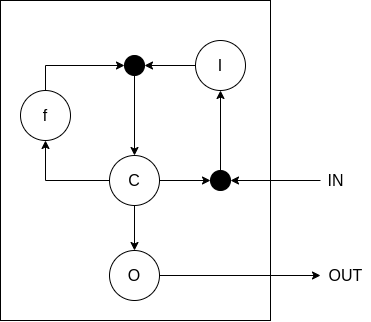
\includegraphics[scale=0.9]{lstm_with_forget_gate_schema.png}}
	\caption{Komórka pamięci w architekturze LSTM z bramką zapominania}
\end{figure}
\FloatBarrier
\newpage
\subsection{Architektura GRU}

Architektura Gated Recurrent Unit (GRU) została zaproponowana przez K. Cho w 2014 roku \cite{https://doi.org/10.48550/arxiv.1406.1078}. Oryginalnie została zaprojektowana do pracy w sieciach typu enkoder-dekoder do tłumaczenia tekstu jako alternatywa dla używanych wcześniej komórek z funkcją aktywacji tangens hiperboliczny. Decyzja o próbie wykorzystania jednostki rekurencyjnej działającej na bramkach była motywowana sukcesem sieci LSTM.

W porównaniu do architektury Long Short-Term Memory Gated Recurrent Unit jest prostsza do zaimplementowania i mniej wymagająca obliczeniowo. Dzieje się tak dzięki zmniejszeniu ilości bramek kontrolujących pamięć komórki. Podczas gdy LSTM do poprawnego działania wymaga użycia trzech bramek (wejściowej, wyjściowej i zapominania) to wewnątrz jednostki GRU występują jedynie dwie bramki (aktualizacja i reset). 

\begin{figure}[!ht]
	\centering
	\makebox[0pt]{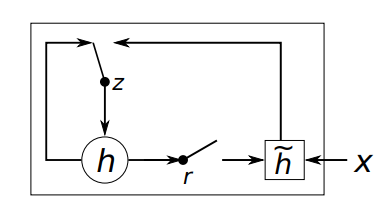
\includegraphics[scale=1]{gru_schema.png}}
	\caption{Komórka pamięci w architekturze GRU}
\end{figure}
\FloatBarrier

Na powyższym rysunku przedstawiony jest schemat komórki GRU, gdzie stan komórki w obecnym kroku czasowym $h$ zmienia się w $\widetilde{h}$. Widoczne są również bramki resetu $r$ i aktualizacji $z$. 

Bramka reset (reset gate) decyduje czy poprzedni wewnętrzny stan komórki powinien być zachowany czy wyrzucony. Jej wartość w j-tej komórce w warstwie wyznaczamy ze wzoru:
\begin{equation}
	r_j = \sigma([W_rx]_j + [U_rh_{t-1}]_j),
\end{equation} 
gdzie $W_r$ i $U_r$ to macierze wag, których wartości są wyznaczane w trakcie uczenia sieci. Przy takich założeniach można zauważyć, że jeżeli wartość bramki reset będzie bliska zeru to stan komórki będzie często usuwany.

Bramka aktualizacji (update gate) decyduje natomiast ile stanu z poprzedniego kroku czasowego należy zapamiętać w obecnym kroku. Wartość bramki w j-tej komórce warstwy wyznaczamy ze wzoru:
\begin{equation}
	z_j = \sigma([W_zx]_j + [U_zh_{t-1}]_j),
\end{equation} 
gdzie $W_z$ i $U_z$ to macierze wag analogiczne do tych występujących w bramce resetu. 

Wiedząc w jaki sposób zachowują się oba typy bramek oraz biorąc pod uwagę, że macierze $W_z, W_r, U_z, U_r$ są wyznaczane w trakcie uczenia można wysunąć kilka obserwacji. Dualizm bramek powinien prowadzić do jednej bramki będącej znacznie bardziej aktywnej od drugiej. Zjawisko to można rozumieć jako specjalizację komórek warstwy, gdzie te z aktywnymi bramkami resetu odpowiadają za pamięć krótkotrwałą, a te z aktywną bramką aktualizacji odpowiadają za pamięć długoterminową. Pamiętając, że aktywność każdej bramki jest dopasowywana dla każdej komórki w procesie uczenia możemy założyć, że podział komórek na pamięć krótkotrwałą i długotrwałą będzie w wytrenowanej sieci rozłożony w sposób optymalny. Rozumiemy przez to, że jeżeli dane treningowe na przykład nie wykazywały długofalowych trendów, a były bardziej chaotyczne i często zmieniające się to po procesie uczenia powinny dominować komórki z aktywną bramką resetu.
\subsection{Indeks Willmott'a}

\newpage
\section{Przygotowanie zbioru danych}
Odpowiednie dane są niezbędne do prób zbadania użyteczności rekurencyjnych sieci neuronowych do predykcji szeregów czasowych. Z tego powodu stworzeniu badawczo ciekawych szeregów czasowych przeznaczona została adekwatna ilość czasu. Przeanalizowano wiele możliwych zbiorów danych aby ich użyć do zbudowania szeregów czasowych. Ostatecznie podjęta została decyzja o połączeniu danych klimatycznych agregowanych przez Instytut Meteorologii i Gospodarki Wodnej oraz danych o zanieczyszczeniu powietrza zbieranych przez Główny Inspektorat Ochrony Środowiska. Oba te zbiory, sposób połączenia ich w szereg czasowy i napotkane trudności zostaną opisane w tym rozdziale. 

\subsection{Baza danych Instytutu Meteorologii i Gospodarki Wodnej}
Instytut Meteorologii i Gospodarki Wodnej to instytucja zajmująca się prognozowaniem pogody i sporządzaniem ekspertyz meteorologicznych. Cel ten jest realizowany między innymi poprzez przeprowadzanie systematycznych pomiarów i obserwacji korzystając z sieci stacji pomiarowych \cite{imgwTask}. Ten aspekt działalności Instytutu implikuje istnienie obszernej bazy danych pomiarowych, które są udostępniane publicznie ponieważ celem Instytutu jest służba społeczeństwu. Ten zbiór danych pomiarowych został wykorzystany do budowy szeregów czasowych. 

Publicznie dostępne są dane klimatyczne od 1951 roku do chwili obecnej. Są one udostępniane w formie dwóch plików csv dla każdego miesiąca roku. Dane w obu plikach mają analogiczną strukturę wyglądającą następująco:
\begin{center}
	\begin{tabular}{|c|c|c|c|c|c}
		Kod stacji & Nazwa stacji & Rok & Miesiąc & Dzień & Wyniki pomiarów...
	\end{tabular}
\end{center}
W kolejnych wierszach są zapisane informacje o pomiarach z jednej stacji z całego miesiąca, potem następnej i tak dalej. Ponieważ wyniki pomiarów z obu plików mogą nieść znaczenie w procesie predykcyjnym podjęta została decyzja o korzystaniu z danych zapisanych w obu plikach. Biorąc pod uwagę oba pliki w bazie danych agregowane są wyniki pomiarów: 
\begin{itemize}
	\item Średniej dobowej temperatury [$\degree C$]
	\item Średniej dobowej wilgotności względnej [\%]
	\item Średniej dobowej prędkości wiatru [$\frac{m}{s}$]
	\item Średniego dobowego zachmurzenia ogólne [oktany]
	\item Maksymalnej temperatury dobowej [$\degree C$]
	\item Minimalnej temperatury dobowej [$\degree C$]
	\item Temperatura minimalnej przy gruncie [$\degree C$]
	\item Suma dobowej opadów [$mm$]
	\item Rodzaju opadu [S (Śnieg) /W (Deszcz)]
	\item Wysokości pokrywy śnieżnej [$cm$]
\end{itemize}
Dla każdego pomiaru jest zapisywany status tego pomiaru pozwalający stwierdzić czy został on przeprowadzony poprawnie i czy dane zjawisko występowało w danym dniu. W wykorzystywanych danych z okresu 2001-2020 nie było przypadku błędnego pomiaru co pozwala wierzyć w dokładność danych i skrupulatność przeprowadzanych obserwacji. 

\subsection{Baza danych Głównego Inspektoratu Ochrony Środowiska}
Główny Inspektorat Ochrony Środowiska to instytucja powołana 27 kwietnia 2001 roku \cite{giosStart}. Jako część swojej misji określa ona mierzenie stanu środowiska oraz udostępnianie wyników tych pomiarów społeczeństwu \cite{giosMission}. Ten aspekt działalności Inspektoratu gwarantuje istnienie dużej bazy wyników pomiarów danych dotyczących poziomu zanieczyszczeń powietrza, które mogą zostać wykorzystane do tworzenia szeregów czasowych. 

Główny Inspektorat Ochrony Środowiska jest instytucją znacznie młodszą o Instytutu Meteorologii i Gospodarki Wodnej, więc dane agregowane przez Inspektorat nie będą dotyczyć tak długiego okresu czasu jak dane Instytutu. Jako że Główny Inspektorat Ochrony Środowiska jest instytucją względnie młodą to w jego początkowych stadiach nie monitorował on wielu różnych typów zanieczyszczeń oraz nie posiadał szerokiej sieci punktów pomiarowych. W trakcie jego rozwoju dochodziło również do zmian w formacie udostępnianych danych. Czynniki te musiały być brane pod uwagę w trakcie pracy z udostępnianymi przez niego danymi. 

Dane te są udostępniane w formie plików formatu xlsx, gdzie dla każdej substancji zanieczyszczającej tworzony jest osobny plik z wynikami pomiarów. Co do zasady struktura danych prezentuje się następująco:
\begin{center}
	\begin{tabular}{|c|c|c}
		Data wykonania pomiaru & Kod stacji 1 & Kod stacji 2 ...
	\end{tabular}
\end{center}
Różne czynniki zanieczyszczające mają również różne rozdzielczości czasowe, dla niektórych jest rozdzielczość godzinna, dla innych dobowa, dla niektórych są dostępne obie. 

Ilość badanych substancji zanieczyszczających powietrze fluktuuje w czasie. W pierwszym roku, dla którego dostępne są dane, mianowicie roku 2000 mierzone były:
\begin{itemize}
	\item Średnie dobowe stężenie Benzo(a)pirenu w pyle PM10
	\item Średnie dobowe stężenie Benzenu
	\item Średnie dobowe stężenie Kadmu w pyle PM10 
	\item Średnie dobowe stężenie Niklu w pyle PM10
	\item Godzinne stężenie Dwutlenku azotu
	\item Średnie dobowe stężenie Dwutlenku azotu
	\item Godzinne stężenie mieszaniny Tlenku azotu i Dwutlenku azotu
	\item Godzinne stężenie Ozonu
	\item Średnie dobowe stężenie pyłu PM10
	\item Godzinne stężenie Dwutlenku siarki
	\item Średnie dobowe stężenie Dwutlenku siarki
\end{itemize}
W kolejnych latach liczba badanych czynników zanieczyszczających oraz rozdzielczość czasowa tych badań znacząco wzrastała, jednak aby zachować możliwość budowy jak najdłuższego szeregu czasowego podjęta została decyzja na braniu pod uwagę jedynie polutantów występujących w wynikach pomiarów ze wszystkich lat działania Inspektoratu. 


Nie bez znaczenia jest również fakt, że ilość stacji badających różniła się znacznie pomiędzy różnymi substancjami. Ostatecznie wybrane zostało używanie jedynie średniego dobowego stężenia pyłu PM10, jako że był on badany przez największą ilość stacji przez najdłuższy możliwy czas. Czynniki te miały duży wpływ na proces budowania jednego szeregu czasowego na podstawie obu opisanych zbiorów danych, który zostanie opisany w dalszej części pracy.

\subsection{Tworzenie szeregów z obu źródeł danych}
Podjęta została decyzja o połączeniu obu źródeł danych w jeden szereg czasowy aby utworzony szereg był badawczo ciekawy. Celem tego działania było umożliwienie predykcji stężenia pyłu PM10 na podstawie danych klimatycznych, ponieważ zdaje się mieć to odzwierciedlenie w rzeczywistości.

Różnice w sieciach stacji pomiarowych Instytutu Meteorologii i Gospodarki Wodnej oraz Głównego Inspektoratu Ochrony Środowiska stanowiły poważny problem w próbie połączenia ich w jeden spójny szereg czasowy. Brak uwzględnienia tego ograniczenia doprowadziłby do całkowitego braku sensownego kontekstu geograficznego w otrzymanym szeregu czasowego. Problem ten został rozwiązany poprzez przygotowywanie osobnych szeregów czasowych dla wybranych stacji Instytutu i Inspektoratu o podobnym położeniu geograficznym. Sposób tworzenia takiego szeregu zostanie przedstawiony na podstawie Krakowa, następnie przedyskutowany zostanie problem tworzenia większej ilości takich szeregów. 

\subsubsection{Tworzenie szeregu dla Krakowa}
Stacja pomiarowa Instytutu Meteorologii i Gospodarki Wodnej w Krakowie posiada jedną stację pomiarową w Krakowie, której wyniki zostały ujęte w danych klimatycznych wykorzystywanych w tej pracy. Natomiast Główny Inspektorat Ochrony Środowiska w okresie będącym tematem zainteresowania tej pracy posiadał wiele różnych punktów pomiarowych w Krakowie. Punkty te często pojawiały się w środku okresu 2000-2020, zmieniały swoje położenie, przestawały prowadzić pomiary lub robiły przerwę w rejestrowaniu zanieczyszczeń na kilka lat. Z tego powodu nie można było skorzystać z wyników każdej ze stacji pomiarowych Instytutu jako zalążka szeregu czasowego bez jego niepotrzebnego skrócenia lub przerw utrudniających analizę. Dodatkowo ponieważ stacje GIOŚ znajdowały się w różnych częściach Krakowa zestawianie ich z jednym punktem pomiarowych IMGW prowadziłoby do szeregu niekoniecznie poprawnie osadzonego geograficznie. Warto również zauważyć, że niektóre stacje pomiarowe zanieczyszczenia powietrza były w obszarach z dużą ilością ruchu samochodowego, inne natomiast w obszarach ze zdecydowanie mniejszym poziomem ruchu samochodowego w okolicy. Takie rozłożenie punktów pomiarowych mogłoby sprawić, że szereg powstały na podstawie danych z jednej stacji IMGW i jednej stacji GIOŚ mógłby być niepoprawny. Jego niepoprawność łatwo zrozumieć na przykładzie, w którym do predykcji zanieczyszczenia nad bardzo ruchliwą ulicą korzystamy jedynie z danych klimatycznych z całkowicie innej części. Taka predykcja najpewniej byłaby wychwycić pewne trendy (np. ludzie częściej korzystający z samochodów w zimie), lecz nie byłyby to kompletne dane potrzebne do przewidywania. Pomijałoby to również wahania warunków pogodowych w różnych częściach miasta, które również mogą wpływać na zanieczyszczenie powietrza.

Aby rozwiązać powyższe problemy stworzony został szereg oparty na danych klimatycznych dostarczanych przez Instytut Meteorologii i Gospodarki Wodnej dla Krakowa oraz średnią arytmetyczną stężenia pyłu PM10 rejestrowanego przez punkty pomiarowe Głównego Inspektoratu Ochrony Środowiska znajdujące się w Krakowie. Takie podejście pozwoliło na stworzenie badawczo interesującego szeregu czasowego, który operował na średnich wartościach zanieczyszczeń w całym Krakowie bez przerw w pomiarach lub błędów. 
Operowanie na średnich wartościach zanieczyszczeń z dużych miast ma również dodatkową zaletę w eliminacji potrzeby troski o bardzo dokładne powody, dla których poziom zanieczyszczeń możne się różnić w takim miejscu. Jako takie powody można przedstawić między innymi: 
\begin{itemize}
	\item Poziom przewietrzania badanego obszaru (dostępność odpowiednich korytarzy powietrznych dla kierunku wiatru w danym dniu, wysokość zabudowy itd.)
	\item Poziom ruchu ulicznego w badanym obszarze (płynność ruchu, dostępność alternatywnych form komunikacji, itd.)
	\item Sposób ogrzewania budynków (dostępność sieci ciepłowniczej, poziom zamożności społeczności lokalnej, itd.)
\end{itemize}
Powodów takich można wymienić znacznie więcej, widzimy jednak, że nie wyeliminowanie potrzeby dbania o nie upraszcza dalsze rozważania. Jest to korzyścią zwłaszcza, celem tej nie jest pracy dokładna analiza powodów występowania zanieczyszczeń powietrza. Dbanie o dokładność szeregu służy tylko upewnieniu się, że przeprowadzane predykcje nie są całkowicie oderwane od rzeczywistości. 

\subsubsection{Tworzenie większej ilości szeregów}
Przy badaniu przydatności rekurencyjnych sieci neuronowych do predykcji czasowych należy skupić się również na potrzebie skalowalności uzyskanych modeli predykcyjnych. Nie ma żadnej gwarancji, że model predykcyjny uzyskujący zadowalające wyniki dla małych zbiorów danych utrzyma zadowalający poziom dokładności predykcji dla zdecydowanie większych zbiorów danych. Fakt ten dla szeregu utworzonego w poprzedniej sekcji oznacza potrzebę stworzenia innych szeregów geograficznych w celu lepszego zrozumienia użyteczności badanych modeli.

W tym celu zbudowane zostały szeregi czasowe dla każdej odpowiadającej sobie geograficznie i czasowo pary punktów pomiarowych z Instytutu Meteorologii i Gospodarki Wodnej oraz Głównego Inspektoratu Ochrony Środowiska. W przypadkach, gdzie występowały wiele punktów mierzących stężenie pyłu PM10 przeprowadzano uśrednianie wyników pomiarów analogicznie do przypadku krakowskiego. Mniejsza uwaga została również poświęcona potrzebie ciągłości szeregu, jako że braki w pewnym fragmencie czasu były ,,przykrywane'' przez inne szeregi. Korzystając z takiej metodologii sporządzone zostały szeregi dla wszystkich sensownych par punktów pomiarowych obu instytucji.
\section{Przeprowadzone badania}
adsfjkhldsfh;dsaf
\subsection{Porównanie wydajności modeli predykcyjnych}
\subsubsection{Regresja liniowa}
\subsubsection{Drzewa decyzyjne}
\subsubsection{Prosta sieć rekurencyjna}
\subsubsection{Sieć rekurencyjna typu LSTM}
\subsubsection{Sieć rekurencyjna typu GRU}
\subsection{Badanie skalowalności modelu GRU}

\section{Otrzymane wyniki}
\subsection{Porównanie wydajności modeli predykcyjnych}
\subsubsection{Regresja liniowa}
\subsubsection{Drzewa decyzyjne}
\subsubsection{Prosta sieć rekurencyjna}
\subsubsection{Sieć rekurencyjna typu LSTM}
\subsubsection{Sieć rekurencyjna typu GRU}
\subsection{Badanie skalowalności modelu GRU}adsfds

\section{Wnioski}
sera
\printbibliography

\end{document}